\documentclass[cclicense]{hmcthesis}

\usepackage{util}
\usepackage{math}

\usepackage{extarrows}
\usepackage{kbordermatrix}

\usepackage{makeidx}
\makeindex

\newcommand*{\x}[1]{\ensuremath{X^{(#1)}}}
\providecommand*{\xs}{\mathcal X}
\providecommand*{\ms}{\mathcal M}
\providecommand*{\ns}{\mathcal N}
\providecommand*{\N}{\mathbb{N}}
\newcommand*{\vbar}{\;\big\vert\;}
\DeclareMathOperator*{\argmax}{arg\ max}

\newcommand*{\mle}{\mathrm{mle}}
\newcommand*{\emp}{\mathrm{emp}}

\numberwithin{equation}{chapter}
\numberwithin{thmcounter}{chapter}

\title{Algebraic Methods for Log-Linear Models}
\author{Aaron Pribadi}
\thesisyear{2012}
\advisor{Michael Orrison}
\reader{Weiqing Gu}

\begin{document}

\frontmatter

\maketitle

\tableofcontents


\chapter{Abstract}
    This will be an abstract.

\chapter{Acknowledgements}
    There will be acknowledgements.

\mainmatter

\chapter{Introduction}

    Discrete data allows us to model the world in almost the simplest way
    possible.  Observations then label things and put them into categories:
    ``This ice cream is green and has sprinkles.''  These procedures appear on
    the surface to be very simple, but the simplicity conceals a deep well of
    difficult problems of intensely practical importance.  The flood of data
    that we cannot yet use as well as we would like increases every year.
    Problems surrounding
    \begin{itemize}\noparspace
    \item genomic sequences,
    \item image recognition,
    \item natural language processing
    \item voting data,
    \item product recommendation,
    \end{itemize}
    and so on are active areas of research driven by real-world concerns.

    Questions arising from the analysis of discrete data pose many challenges,
    but at the same time offer rich mathematical structures.  There are two
    complementary hopes.  The first is that ideas from `pure' mathematics,
    particularly geometry and algebra, can offer guiding principles and
    effective techniques for the analysis of data.  The second is that practical
    problems will in turn suggest avenues for further exploration of intrinsic
    interest.

    We take a look at log-linear models, a particular class of models that
    interact particularly well with ideas from geometry and algebra.  While
    these models make simplistic assumptions, many standard techniques from the
    analysis of discrete data already fall under its umbrella.  As the name
    suggests, log-linear models are in some sense linear.  A linear structure,
    as is often the case, is a shortcut to tractability.  Furthermore, linearity
    allows concerns about symmetry and invariance to be more readily exploited.
    Within this framework, ideas from representation theory and even algebraic
    geometry can be brought to bear on questions of model selection.

    Blah blah

\chapter{Discrete Models}

    \section{Discrete Data}

    A random variable (from an elementary standpoint) is either 
    \begin{itemize}\noparspace
    \item discrete, when its sample space is countable, or
    \item continuous, when its sample space is a subset of $\R^n$.
    \end{itemize}
    The first case is the one that we consider.  In particular, we usually take
    the relevant sample spaces to be finite.  Because we can then deal with
    finite-dimensional spaces, this simplifies many ideas.

    Another fundamental assumption is that repeated observations are independent and
    identically distributed random variables.  That is, the observations $\x 1,
    \ldots, \x m$ are random variables, and each is distributed according to the
    same underlying probability distribution, $\x i \sim p$.  Given an observed
    set of values for the $\x i$, a basic objective is to estimate the
    underlying probability distribution $p$.

    Let each $\x i$ take a value from the sample space $\xs$.  Throughout, we
    assume that $\xs$ is a finite set.  Because the order of the observations
    does not matter, we can summarize the observations with the counts
    \begin{equation*}
        u(x) = \pdel{\text{the number of $i$ for which $\x i = x$}}
    \end{equation*}
    for $x \in \xs$.  If the number of states $|\xs|$ is small relative to the
    number of samples $m$, then the empirical distribution
    \begin{equation}
        p_\emp(x) = \frac{u(x)}{m}
        \label{eq:empirical}
    \end{equation}
    is a useful estimate of the true distribution $\x i \sim p$.

    It is sometimes the case that $|\xs|$ is very large.  Without a
    correspondingly large number of samples, the empirical distribution $p_\emp$
    may not adequately capture the underlying distribution $p$.  Such sample
    spaces arise naturally in a variety of situations, especially when
    combinatorial processes are involved.
    \begin{itemize}
    \item Multivariate data occurs when multiple things are observed at once.
    The sample space is a cartesian product
    \[
        \xs = \xs_1 \times \cdots \times \xs_k
    \]
    of several finite sets.  The component space $\xs_i$ for each variate can be
    the assignment of a label to each observation.  For example, a person can
    have an eye color, a handedness, a gender, a political affiliation, and many
    more characteristics.
    
    If each variate has approximately the same number of possible values, then
    the size of the sample space is exponential in the number of variates.  

    An excellent and comprehensive reference for the statistical analysis of
    multivariate data is the book by \citet{DMA}.

    \item Group-valued data occurs when discussing the arrangements of a system.
    For example, voters in an election could be asked to rank $n$ candidates.
    The sample space is then the symmetric group $\xs = S_n$.  If there is no
    special base point of the sample space to call the identity of the group,
    another choice is to consider the sample space as a principal homogeneous
    space.

    Clearly, it is rather easy to construct simple examples with large numbers
    of possible outcomes, e.g. $n!$ for the symmetric group.
    \end{itemize}
    For the empirical distribution to produce a good estimate of the underlying
    distribution, a prohibitively large number of samples is required.

    In order to analyze data with a large number of states, it is often fruitful
    to restrict which distributions we consider.  One goal is to use the
    structure of the underlying space of states in order to better analyze data.

    \begin{example}[Binary Voting]
        The UCI database \citep{UCIData} contains a large number of data sets
        useful for the evaluation of machine learning techniques.  The
        Congressional Voting Records data set contains Congressional voting
        records on a number of key issues.
        \begin{figure}[H]
            \centering
            \begin{verbatim}
            1) democrat   n y y n y y n n n n n n y y y y
            2) republican n y n y y y n n n n n y y y n y
            3) democrat   y y y n n n y y y n y n n n y y
            4) democrat   y y y n n n y y y n n n n n y y
            5) democrat   y n y n n n y y y y n n n n y y
            \end{verbatim}
            \vspace{-1.5\baselineskip}
            \caption{A few points from the Congressional Voting Records
            data set.}
        \end{figure}
        \noindent Ignoring missing values, e.g. where representatives did not
        vote, each variate has two possible values, either $\{\texttt{democrat},
        \texttt{republican}\}$ or $\{\texttt{yes}, \texttt{no}\}$.  Thus, the
        sample space may be written as $\xs = \{0, 1\}^7$, the set binary
        strings with 7 bits.  As $|\xs| = 2^{17} = 131072$ is a large number,
        some assumptions about potential distributions are needed to make sense
        of the data.
        \label{ex:binary-voting}
    \end{example}


    \section{The Simplex and Statistical Models}

    We take a geometric view of statistical models.  The formulation of
    statistical objects in terms borrowed from other parts of mathematics allows
    statistical problems to be attacked with a large range of useful tools.  The
    adoption of this perspective is in large part influenced by the lecture
    notes by \citet{DSS08}, which summarizes recent progress in using the tools
    of algebraic geometry for statistics.

    A probability distribution on a finite set $\xs$ can be thought of as a
    real-valued function $p \in L(\xs)$ subject to the restrictions that
    $\sum_{x\in \xs} p(x) = 1$ and that $p(x) \ge 0$ for all $x \in \xs$.  The
    function $p$ is the probability mass function.  Finite sets are particularly
    convenient because we can always work with a probability mass function, and
    because the probability mass function is always embedded in an ambient
    finite dimensional vector space.  The space of all distributions on $\xs$ is
    a geometric object.
    
    \begin{definition} 
        \index{simplex}
        The \emph{standard simplex} of dimension $n$ is the subset
        \[
            \Delta_n = 
            \left\{(p_1, \ldots, p_{n+1}) \in \R^{n+1} \vbar 
            \sum_{i=1}^{n+1} p_i= 1, p_i \ge 0 \right\} 
        \]
        of $\R^{n+1}$.  If the appropriate dimension is either clear in context
        or irrelevant, then we may write $\Delta$, omitting the subscript.
    \end{definition}

    The simplex is a generalization of an equilateral triangle.  Low-dimensional
    simplices are familiar shapes; $\Delta_0$ is a point, $\Delta_1$ is a line
    segment, $\Delta_2$ is a triangle, and $\Delta_3$ is a tetrahedron.

    \begin{figure}[H]
        \centering
        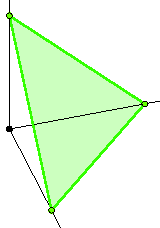
\includegraphics[scale=1]{2-simplex.pdf}
        \caption{The 2-simplex.}
    \end{figure}

    There is a one-to-one correspondence between probability distributions on
    the set $\xs = \{x_1, \ldots, x_{n+1}\}$ and points in the simplex
    $\Delta_n$; the probability $p(i)$ is equal to the value of the coordinate
    $p_i$.  We therefore identify the two concepts with each other.
    Because the space of all probability distributions is a geometric
    object, it is easy to talk about specific families of probability
    distributions.

    \begin{definition}
    A \emph{statistical model} is a subset $\ms \subset \Delta$ of the
    probability simplex.  A \emph{parametrized model} $\ms$ with parameter space
    $\Theta$ is specified by a surjective map $\Theta \to \ms$.  We usually
    write $p_\theta$, with $\theta \in \Theta$, to denote a distribution from a
    parametrized model.
    \end{definition}

    Many statistical models have been studied and employed for the analysis of
    data, and the selection of an appropriate model is a delicate question.  In
    Section~\ref{sec:linear-models} we introduce a family of models with
    convenient properties.

    In an ideal situation, there is a hypothesis for an underlying mechanism
    producing the observable results.  In that case, a particular choice of
    model is easy to justify.

    \begin{example}[Binomial Model]

        The distribution $\mathrm{Binom}(N, \alpha)$ models the number of heads
        produced by $N$ independent `coin tosses', where \mbox{$0 \le \alpha \le
        1$} is the probability that a single toss produces a head.  It is
        defined by the probability density function
        \[
            p_\alpha(k) = {N \choose k} \alpha^k(1-\alpha)^{n-k}.
        \]
        for $k \in \{0, \ldots, N\}$.  The map $\alpha \mapsto p_\alpha$
        determines a parametrized statistical model.  The statistical model is a
        curve, i.e. a one-dimensional subset of the simplex.  

        The model $\mathrm{Binom}(2, \alpha)$ simulates two coin flips.  The
        three coordinates of a point in the model measure the probabilities that
        zero, one, and two heads will occur, respectively.

        \begin{figure}[H]
            \centering
            \vspace*{-0.2cm}
            \scalebox{1}{ 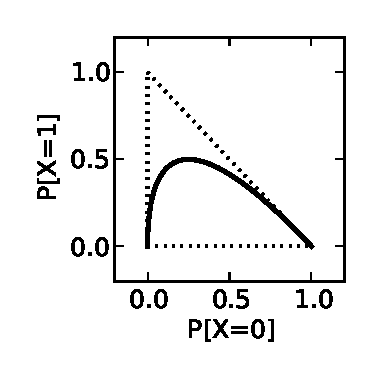
\includegraphics[scale=0.7]{images/binomial.pdf} }
            \vspace*{-0.5cm}
            \caption{The binomial model for $N=2$. Make this 3-D?}
            \label{fig:binomial}
        \end{figure}

        \noindent As the parameter $\alpha$ varies over $[0,1]$, the statistical
        model traces out the curve 
        \[
            \alpha \longmapsto \big((1-\alpha)^2, 2\alpha(1-\alpha), \alpha^2\big)
        \]
        in the simplex $\Delta_2$ (see Figure~\ref{fig:binomial}).  

        If we knew that a coin was being flipped twice and did not know the
        odds of the coin, then the model $\alpha \mapsto \mathrm{Binom}(N,
        \alpha)$ would be an appropriate choice for the situation.
    \end{example}

    \begin{example}[Multivariate Independence]
        The independence model on a sample space $\xs = \xs_1 \times \cdots
        \times \xs_k$ assumes that each variate is independent.  For a
        distribution $p$ on $\xs$, the variates are said to be independent if
        $p$ factors as
        \[
            p(x) = p_1(x) \cdots p_k(x)
            \qquad
            \text{where}
            \qquad
            p_i(x) = \sum_{y_i = x_i} p(y) % \stackrel{y \in \xs}{x_i = y_i}} p(y)
        \]
        for all $x = (x_1, \ldots, x_k) \in \xs$.  Each factor $p_i(x)$ is a
        function only of the $i$th component of $x$.  Despite this simplistic
        assumption, the independence model is surprisingly effective in many
        situations, e.g. for naive Bayes classifiers.  
        
        The map 
        \begin{align*}
        \Delta_{|\xs_1|-1} \times \cdots \Delta_{|\xs_k|-1} 
        &\to \Delta_{|\xs| - 1} \\
        (p_1, \ldots, p_k) &\mapsto p_1 \cdots p_k
        \end{align*}
        gives a one-to-one parametrization of the independence model.  Counting
        dimensions indicates that the independence model imposes strict
        limitations on potential distributions.  The parameter space has
        dimension
        \[
            \dim 
            (\Delta_{|\xs_1|-1} \times \cdots \Delta_{|\xs_k|-1})
            =
            |\xs_1| + \cdots + |\xs_k| - k
        \]
        whereas the space of all distributions on $\xs$ has dimension 
        \[
            \dim(\Delta_{|\xs| - 1})
            =
            |\xs_1| \cdots |\xs_k| - 1.
        \]
        If the variates are binary, as in Example~\ref{ex:binary-voting}, then the
        model has dimension $k$ and the whole simplex has dimension $2^k - 1$.
        The latter grows much more rapidly with increasing $k$ than the former.
        \label{ex:independence1}
    \end{example}
    
\section{Likelihood and Model Complexity}
    In the analysis of data, there is a tension between how well an explanation
    fits the observed data, and how well such an explanation can be expected to
    generalize to new data.  While we do not explore all nuances of this
    trade-off, we do introduce a few fundamental concepts.

    One way to measure how well a distribution matches data is to ask the
    question, ``How likely is the data, given the distribution?''  A maximum
    likelihood estimate quantifies whether a model contains distributions that
    match well.

    Let $\ms = \{p_\theta : \theta \in \Theta\}$ be a parametrized statistical
    model.  Suppose that some data $Z = \{z_1, \ldots, z_m\}$ are observed.  It
    is generally assumed that the data has been drawn from independent and
    identically distributed samples following an unknown true distribution from
    the model.from the model.
    
    \begin{definition}
    The \emph{likelihood function} of $\theta \in \Theta$ given the data $Z$ is
    \[
        L(\theta; Z) = \prod_{i=1}^n p_\theta(z_i).
    \]
    It is the probability that the observed data $Z$ would occur if the samples
    followed $p_\theta$.  Oftentimes, the \emph{negative log-likelihood}
    \begin{equation}
        -l(\theta; Z) = -\log L(\theta; Z) = -\sum_{i=1}^n \log p_\theta(z_i).
        \label{eq:negloglik}
    \end{equation}
    is used in lieu of the likelihood.  The negative log-likelihood is useful
    because the contributions to $-l(\theta; Z)$ from the observations $z_i$ are
    additive and each acts as a `penalty' or `loss'.
    \end{definition}
    \begin{definition}
    The \emph{maximum likelihood estimate} of the true parameter is the
    parameter 
    \[
        \theta_\mle = \argmax_{\theta \in \Theta} L(\theta; Z)
    \]
    that maximizes the likelihood of the data, or equivalently that minimizes
    the negative log-likelihood of the data.  In some cases, we identify the
    parameter $\theta$ with the distribution $p_\theta$. The term `maximum
    likelihood estimate' then refers to the distribution $p_\mle$ that maximizes
    the likelihood, given a choice of model.
    \end{definition}

    \begin{note}
        The fact that a maximum likelihood estimate might not exist or might not
        be unique is tacitly ignored.  Indeed $\{L(\theta; Z) \mid \theta \in
        \Theta\}$ might be an open set, and the map $\theta \mapsto L(\theta;
        Z)$ might not be surjective.  In applications with real data, it is
        often the case that a precise maximum likelihood estimate is not
        necessary, and that an approximate value is sufficient.
    \end{note}

    The distribution $p_\mle$ from the maximum likelihood estimate is the best
    one possible from the model.  Notice that if $\ms \subset \ns$ are two
    nested statistical models, then the maximal likelihood from $\ms$ is less
    than or equal to that from $\ns$.  Thus the size of the model determines how
    good of a distribution is possible.

    \begin{example}
        Suppose that the model does not restrict distributions at all, i.e.
        that the model is the whole simplex.  Then the maximum likelihood
        estimate is the empirical distribution $p_\emp$ as in
        \eqref{eq:empirical}.
    \end{example}

    \begin{example}[Multivariate Independence]
        Recall the independence model from Example~\ref{ex:independence1}.  The
        maximum likelihood estimate for the independence model is
        \[
            p_\mle(x) = \frac{u_1(x_1)}{m} \times \cdots \times \frac{u_k(x_k)}{m}
        \]
        where $x = (x_1, \ldots, x_k)$, $m$ is the number of samples, and
        $u_i(x_i)$ is the number of times that the $i$th variate of the
        observation is $x_i$.  In other words, we get a maximum likelihood
        estimate of each variate separately with its empirical distribution, and
        take the product distribution.
    \end{example}

    A larger model is deemed to contain more `complex' distributions.  The
    trade-off is that a larger model allows for probability distributions that
    fit the observed data better, but that might not generalize as well to
    subsequent observations.  This trade-off between model complexity and
    predictive power can be approached in a number of ways, and is explored in
    the standard literature.  Chapter 7 of the book \citet{EOSL} is one
    reference.  
    
    There are at least two common methods to limit model complexity.
    \begin{itemize}
    \item We can require that the estimated distribution $p$ is contained within
    some model $\ms \subset \Delta$.
    \item We can minimize $-l(p) + \pi(p)$, the negative log-likelihood with an
    additional penalty term measuring the complexity of $p$.
    \end{itemize}
    Two criteria with complexity penalties are the Akaike information criterion
    and the Bayesian information criterion, defined
    \begin{align*}
        \mathrm{AIC} &= -2\,l(p_\mle) + 2d \\
        \mathrm{BIC} &= -2\,l(p_\mle) + (\log m) d
    \end{align*}
    where $-l(p_\mle)$ is the log-likelihood of the maximum likelihood estimate
    as in \eqref{eq:negloglik}, $d$ is the dimension of the parameter space
    $\Theta$, and $m$ is the number of samples.  These two criteria have
    different motivations, which are described in the above reference.

\section{Log-Linear Models}
    \label{sec:linear-models}
    
    The selection of distributions can be treated as a problem in function
    estimation.  From the data we construct the empirical distribution \mbox{$p_\emp
    \in L(X)$}, and we wish to find another function $p \in L(X)$ that
    approximates $p_\emp$ subject to some set of restrictions.  
    
    The structure of $L(X)$ as a linear space suggests one method of
    approximation.  One can expand $p_\emp$ in terms of a basis $B = \{v_1,
    \ldots, v_n\}$ of $L(X)$, $p_\emp = \sum_{i=1}^n \lambda_i v_i$.  Any subset
    $C \subset B$ of the basis elements yields an approximation $\sum_{v_i \in
    C} \lambda_i v_i$ of $p_\emp$ from the subspace spanned by $C$.  One can
    select the terms with the largest coefficients $\lambda_i$, or, if the basis
    has some natural ordering, can simply truncate the series.

    This method of approximation has at least one drawback, namely that negative
    probabilities are possible.  Dealing instead with log-probabilities is often
    fruitful.  In fact, log-linear models, i.e. discrete exponential families,
    are especially prevalent in the analysis of discrete multivariate data.
    \begin{definition}
        A \emph{log-linear} model $\ms_{V,h}$ is a statistical model of the form
        \[
            \ms_{V,h} = \cdel[\big]{p \in \Delta_{n-1} \:: \log p = (\log p_1, \ldots,
            \log p_n) \in V + h}
        \]
        where $h \in \R^n$, $V$ is a linear subspace of $\R^n$, and $V + h$ is
        an affine subspace.
    \end{definition}

    The usual definition of an exponential family (which need not be over a
    finite sample space) is as follows.
    \begin{definition}
        An \emph{exponential family} over a sample space $\xs$ parametrized by
        $\Theta$ contains distributions of the form
        \[
            p_\theta(x) = 
            \frac 1 {Z(\theta)}
            \exp\pdel*{
                \displaystyle \sum_{i=1}^d \eta_i(\theta)T_i(x) + h(x)
            }
        \]
        where $\eta : \Theta \to \R^d$, $T:\xs \to \R^d$, and $h: \xs \to \R$
        are known functions, and $Z:\Theta \to \R$ is a normalizing constant
        known as the partition function.
    \end{definition}
    An exponential family is a log-linear model when $\xs$ is finite and $\eta$
    is the identity map $\R^d \to \R^d$, as $p_\theta$ is constrained to lie in
    the affine space
    \[
        \mathrm{span}\cdel*{
            (T_i(x_1), \ldots, T_i(x_n)) \:: i \in \{1, \ldots, d\}
        } + h
    \]
    where $h$ is interpreted as a vector in $\R^n$.  

    \begin{example}[Binary Multivariate Independence]
        The independence model with strictly positive probabilities is a
        log-linear model.  We compute this explicitly for the case where the
        sample space is $\xs = \{0, 1\}^2$ and we wish the two bits to be
        independent.  One can verify that a distribution $p$ on $\xs$ is in the
        independence model if and only if $\log p$ is in the row span of the
        matrix
        \[
            \kbordermatrix{
                & 00 & 01 & 10 & 11 \\
                &  1 &  1 &  0 &  0 \\
                &  0 &  0 &  1 &  1 \\
                &  1 &  0 &  1 &  0 \\
                &  0 &  1 &  0 &  1
            }.
        \]
        Notice that the matrix has rank 3, so that the independence model is a
        proper subset of the full simplex.
    \end{example}

\section{Sparsity and Regularization}

    Why are we so keen on cutting down the number of dimensions?  The reason,
    which arises in optimization and statistics, is colorfully termed the \emph{curse
    of dimensionality}.  It is easiest to illustrate problem in another closely
    related setting.

    \begin{example}[Sampling and the Curse of Dimensionality]
        We describe a classification problem with $p$ real-valued features.
        Concretely, say that we want to label points in the $p$-dimensional cube
        $[0, 1]^p$ either \texttt{blue} or \texttt{orange}.  We can sample some
        points in the cube to check their color.  A reasonable assumption is
        that if a point $u$ is \texttt{blue}, then another nearby point $v$
        (where $\|u - v\|$ is small) is probably also \texttt{blue}.  This is
        known as a nearest-neighbor classification algorithm.  
        
        When $p$ becomes large, the volume of a neighborhood around a point
        becomes very small relative to the total volume of the space.  If, say,
        we wanted samples placed on a grid with separations of about $0.1$, then
        we would need about $10^p$ samples.  Filling the whole space requires
        exponentially many samples.
    \end{example}

    In statistical learning, this is also known as the `$p \gg N$' problem,
    where $p$ is the number of features and $N$ is the number of samples.  One
    method for battling the curse of dimensionality is to encourage
    \emph{sparsity}.  Roughly, this means that in a linear problem with many
    parameters, we want the majority of the parameters to be $0$.  
    
    \begin{example}[Linear Regression]
        The term `sparse' arises from linear regression.  In that setting one
        wishes to find a relation $y = Ax$, where $x \in \R^N$, $y \in \R$, and
        $A$ is a linear transformation.  A sparse solution is one where many
        entries of the matrix $A$ are zero, i.e. where $A$ is a sparse matrix.
    \end{example}
    
    Methods that encourage sparsity have been found to perform well in practice.
    In what they call the ``bet on sparsity'', \citeauthor{EOSL} introduce a
    heuristic that explains the importance of sparse methods:
    \begin{quote}
        Use a procedure that does well in sparse problems, since no procedure
        does well in dense problems.
    \end{quote}
    \noindent Essentially, we must assume that we can find important
    low-dimensional spaces, because otherwise estimation of parameters becomes
    very difficult.

    We outline one approach to sparse modeling, the vividly named Lasso, first
    introduced in a paper by \citet{LASSO}.  Consider a model with real
    parameters $\beta_1, \ldots, \beta_n$.  As before the setting is one of
    linear regression, fitting $y = \sum_{i=1}^n \beta_i x_i$.  The idea is to
    minimize
    \[
        \sum_{j=1}^m \pdel*{y_j - \sum_{i=1}^n \beta_i x_i}^2 + \lambda \sum_{i=1}^n
        |\beta_i|
    \]
    given data $\{(x^{(j)}, y^{(j})\}_{j=1}^m$ and some hyperparameter $\lambda
    > 0$.  That is, it minimizes the residual sum of squares with an additional
    penalty term which is a factor of the $L_1$-norm of the parameter vector.
    As the value of $\lambda$ is increased, this approach causes some parameters
    to go to exactly zero, yielding a sparse model.  The usage of the $L_1$ norm
    as a penalty is also known as $L_1$ regularization.  The procedure derived
    from using $L_2$ regularization instead is known as ridge regression; in
    contrast, it does not bring select parameters to zero, but instead reduces
    all parameters at the same time.

    The approach of $L_1$ regularization has also been applied directly to
    log-linear models, in the paper by \citet{SPEC}.  In it, they use a basis
    $\{b_1, \ldots, b_n\}$ for $L(\xs)$ and minimize
    \[
        - \sum_{j=1}^m \log \pdel*{\sum_{i=1}^n \beta_i b(z_j)} + \lambda
        \sum_{i=1}^n |\beta_i| 
    \]
    with data $z_1, \ldots, z_m$ and hyperparameter $\lambda$ fitted by
    cross-validation.

    One thing to keep in mind is that the Lasso and other methods for finding
    sparse models depend on selecting either subspaces of $L(\xs)$ or even a
    full basis beforehand.  Because there are many possible choices for such
    subspaces, one would like to know that the outcome of the procedure is not
    too dependent on arbitrary choices, or that the choice of subspaces is
    somehow natural.


\chapter{Structured Sample Spaces}

\section{An Invariance Principle}
    
    The array of possible models and regularization procedures is large enough
    that some guiding principles are sorely needed.  Symmetries of the sample
    space suggest some requirements.  We shall say that we wish our statistical
    procedures to be invariant under reparametrization.  

    More precisely, depending on the nature of the sample space $\xs$, there are
    permutations $\sigma: \xs \to \xs$ that preserve the structure of $\xs$.
    Such permutations form the automorphism group of the sample space.  In
    essence, the automorphism group describes the admissible ways to re-label
    the data.

    \begin{example}[Binary Multivariate Data]
        Suppose that as in Example~\ref{ex:binary-voting} the data consist of
        voting records of individuals on $n$ binary issues.  The sample space is
        $\{0, 1\}^2$.  A natural choice for the automorphism group is the
        hyperoctahedral group.  The case of binary multivariate data will be our
        primary example, and we will subsequently examine it more closely.
    \end{example}
    
    That is, if there is a permutation $\sigma: \xs \to \xs$ of the sample space
    that preserves the structure of the sample space, then we want the result of
    the statistical procedure performed on the transformed $\sigma(\xs)$ to be
    the same as if it were performed on $\xs$.

    Both the counts $u: \xs \to \N$ and the log-probabilities $\log p$ lie in
    the linear space $L(\xs)$.  When $|\xs|$ is very large, it is useful to
    break up $L(\xs)$ into constituent parts.  This can be a decomposition into
    subspaces, or, if possible, a natural choice of basis.  This
    decomposition should rely on the underlying structure of the space of states
    $\xs$.

    Under the log-linear framework described in Section~\ref{sec:linear-models},
    the permutation $\sigma$ induces a linear automorphism of $L(\xs)$.  If some
    data $\{z_1, \ldots, z_m\}$ indicates that a subspace $V \subset L(\xs)$ is
    of particular importance, then the same procedure with the data
    $\{\sigma(z_1), \ldots, \sigma(x_m)\}$ should similarly indicate the
    subspace $\sigma(V)$.

    Furthermore, if some subspace of $L(\xs)$  is intrinsically important for a
    sample space but without any reference to particular data, that subspace
    should be invariant under permutations $\sigma$.

\section{Homogeneous Spaces}

    Often, $\xs$ exhibits large amounts of symmetry.  In the best case, every
    point in $\xs$ is the same, in some precise way.  A useful geometric
    formulation is that of a homogeneous space.
    \begin{definition}
        A \emph{homogeneous space} is a space $\xs$ together with a transitive
        action of a group $G$ on $\xs$.
    \end{definition}
    Given a choice of any point $x_0 \in \xs$, let $K$ be the stabilizer of
    $x_0$.  Then we can identify the set $\xs$ with the coset space $G / K$.
    Homogeneous spaces usually turn up in the context of Lie groups, with which
    the group action has additional restrictions.

    The choice of group action is usually motivated by the meaning of the set
    $\xs$.  We often want some sort of invariance property, where, for example,
    the order in which we label things to not matter.

\section{Binary Models}

    Let $\xs = \{0, 1\}$ be the space of states consisting of binary strings.
    \[
        \{0, 1\}^n = \{0\cdots00, 0\cdots01, \ldots, 1\cdots11\}
    \]
    
    If we do not have any information about what the value of each bit means,
    there are two types of natural actions:
    \begin{itemize}\nospace
    \item Reordering of the bits.
    \item `Flipping' a bit.
    \end{itemize}
    We formulate these two requirements concretely.  

    \begin{figure}[H]
        \centering
        Put something here!
        \caption{A permutation of the bits.}
    \end{figure}
    
    The two symmetry requirements each specify a permutation of the states $\{0,
    1\}^n$.  If $\mu \in S_n$ reorders the bits, the corresponding permutation
    of the states is
    \begin{align*}
        \{0, 1\}^n &\to \{0, 1\}^n \\
        b_1 \cdots b_n &\mapsto b_{\mu(1)} \cdots b_{\mu(n)}.
    \end{align*}
    A flip of the $k$th bit is the permutation
    \begin{align*}
        \{0, 1\}^n &\to \{0, 1\}^n \\
        b_1 \cdots 0 \cdots b_n 
        &\mapsto
        b_1 \cdots 1 \cdots b_n  \\
        b_1 \cdots 1 \cdots b_n 
        &\mapsto
        b_1 \cdots 0 \cdots b_n
    \end{align*}
    where the $k$th position is modified.  
    
    Let $\sigma: \{0, 1\}^n \to \{0, 1\}^n$ be a permutation of the states.
    Such a permutation `lifts' to an automorphism of $\Delta$, the space of
    probability distributions.  Let $p: \{0, 1\}^n \to [0, 1]$ be a function
    from states to some probability for each state; the function $p$ represents
    a probability distribution, so we say $p \in \Delta$.  Then $\sigma$ acts on
    $\Delta$ with the formula
    \begin{equation}
        (\sigma p)(b_1 \cdots b_n) = p(\inv \sigma(b_1 \cdots b_n)).
        \label{eq:sigma-p}
    \end{equation}
    A model $\ms \subset \Delta$ is said to be invariant under the action of
    $\sigma$ if $p \in \ms$ implies that $\sigma p \in \ms$.  (Invariance is
    actually a bit too strong \ldots)

    The permutations specified by reorderings and flips of bits are elements of
    the symmetric group on $\{0, 1\}^n$.  They generate the group known as the
    hyperoctahedral group $S_2 \wr S_n$.  We will examine the structure of the
    hyperoctahedral more closely in Section~\ref{sec:hyperoctahedral}.

    \eqref{eq:sigma-p} specifies a group action of $S_2 \wr S_n$ on $\Delta$.
    Each automorphism of $\Delta$ given by a group element is invertible, so we
    can interpret the invariance requirement geometrically as
    \[
        \sigma(\ms) = \ms
        \qquad
        \text{for all $\sigma \in S_2 \wr S_n$},
    \]
    that is, the action of every element of the group maps the model to itself.


    The group of interest to us is the hyperoctahedral group.  This group may be
    defined as the automorphism group of the $n$-hypercube or as the wreath
    product $S_2 \wr S_n$.
% Coxeter?
    The first formulation is very concrete, so we describe it first. 

    Each joint state of the $n$ binary random variables can be represented as a
    binary string of length $n$.  That is, the states are
    \[
        \underbrace{
        \underbrace{0\cdots00}_\text{$n$ bits}\;,\;
        0\cdots01,\;
        0\cdots10,\;
        \ldots,\;
        1\cdots11
        }_\text{$2^n$ binary strings}.
    \]
    \begin{definition}
    The \emph{Hamming distance} between two binary strings is the number of
    positions in which the two strings differ.  
    \end{definition}
    For example, the following binary strings of length 4 have Hamming distances
    of 0, 1, and 2.
    \begin{align*}
        0010 &\xleftrightarrow{\quad\text{Hamming distance $0$}\quad} 0010 \\
        0010 &\xleftrightarrow{\quad\text{Hamming distance $1$}\quad} 0110 \\
        0010 &\xleftrightarrow{\quad\text{Hamming distance $2$}\quad} 0100
    \end{align*}
    The hypercube graph uses the Hamming distance to determine its edges.
    \begin{definition}\index{hypercube}
        The \emph{$n$-hypercube} graph has as its vertices the length-$n$ binary
        strings.  There is an edge between two vertices if and only if
        their Hamming distance from each other is 1, that is, if they differ in
        exactly one bit.
    \end{definition}
    The graph distance between any two vertices of the hypercube graph, i.e. the
    minimal number of edges between those two vertices, is the same as their
    Hamming distance.  A look at a picture of a hypercube graph
    (Figure~\ref{fig:hypercube}) makes it clear as to why it is called a
    hypercube.


    \begin{figure}[h]
        \centering
        % http://code.google.com/p/graph-theory-algorithms-book/
        % GPL Documentation Licence

        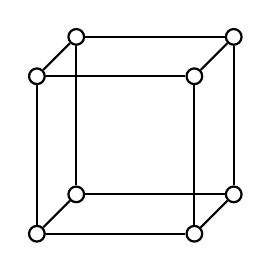
\begin{tikzpicture}
        [nodedecorate/.style={shape=circle,inner sep=2pt,draw,thick},%
          linedecorate/.style={-,thick}]
        %% nodes or vertices
        \foreach \nodename/\x/\y in {1/0/0, 2/2/0, 3/2/2, 4/0/2, 5/0.5/0.5,
          6/2.5/0.5, 7/2.5/2.5, 8/0.5/2.5}
        {
          \node (\nodename) at (\x,\y) [nodedecorate] {};
        }
        %% edges or lines
        \path
        \foreach \startnode/\endnode in {1/2, 2/3, 3/4, 4/1, 5/6, 6/7, 7/8,
          8/5, 1/5, 2/6, 3/7, 4/8}
        {
          (\startnode) edge[linedecorate] node {} (\endnode)
        };
        \end{tikzpicture}

        \caption{The $3$-hypercube graph}
        \label{fig:hypercube}
    \end{figure}
    
    Speaking generally, the symmetries of an object correspond with a group
    action that preserves the structure of the object.  The structure of a graph
    is determined entirely by its edges.
    \begin{definition}
        A \emph{graph automorphism} is a permutation of the vertices of a graph
        that preserves the edges.  That is, a permutation $\sigma: V \to V$ is a
        graph automorphism if for every $(u, v) \in E$, we have $(\sigma(u),
        \sigma(v)) \in E$.
        The \emph{automorphism group} of a graph is the set of all
        automorphisms of a graph with the group operation being composition of
        permutations.
    \end{definition}

    \begin{definition}
        The \emph{hyperoctahedral group} $H_n$ is the automorphism group of the
        $n$-hypercube.
    \end{definition}

    The wreath product is a construction on two permutation groups.
    Essentially, one permutation group shuffles copies of another permutation
    group.  In our example, $S_n$ permutes the binary variables, each of which
    has two states.  The copies of $S_2$ are each attached to one of the
    variables, and flip the values $0$ and $1$.  These copies of $S_2$ are then
    shuffled by the action of $S_n$.  We present a formal definition of the
    wreath product.
    \begin{definition}[\citet{Cam99}]
        Let $H$ and $K$ be permutation groups on the sets $\Gamma$ and $\Delta$
        respectively.  Let $\Omega = \Gamma \times \Delta$.  Think of $\Omega$
        as a fiber bundle over the set $\Delta$, with projection map $(\gamma,
        \delta) \mapsto \delta$; each fiber \mbox{$\Gamma_\delta = \{(\gamma, \delta)
        \mid \gamma \in \Gamma\}$} for fixed $\delta \in \Delta$ is isomorphic to
        $\Gamma$.  Let $B$ be the cartesian product of $|\Delta|$ copies of $H$,
        one acting on each fiber as $H$ acts on $\Gamma$.  Thus $B$ is the set
        of functions from $\Delta$ to $H$ with pointwise operations; the action
        on $\Gamma \times \Delta$ is given by
        \[
            f\cdot(\gamma, \delta) = (f(\delta) \cdot \gamma, \delta)
        \]
        where ($\cdot$) is used to denote group actions.  Let $T$ be a copy of
        the group $K$ permuting the fibers:
        \[
            k \cdot (\gamma, \delta) = (\gamma, k \cdot \delta).
        \]
        Then wreath product $H \wr K$ is defined to be the semidirect product $B
        \rtimes T$.
    \end{definition}

\section{Isotypic Decomposition}
    
    The idea of representation theory is to better understand the structure of a
    group (or algebra) by transferring the problem to the domain of linear
    algebra.  The field of representation theory is very rich, and we only
    introduce a few foundational concepts from the representation theory of
    finite groups.

    \begin{definition}
        A \emph{representation} of a group $G$ is a group homomorphism $\rho: G
        \to GL(U)$ from $G$ to the group of invertible linear transformations on
        a vector space $U$.  
    \end{definition}
    Here, we make the simplifying assumptions that $G$ is a finite group and
    that $U$ is a finite dimensional complex vector space.  It is common to
    identify the group representation $\rho$ with the vector space $U$; we then
    say that $U$ is the group representation.

    Representations of finite groups behave tractably in large part because they
    decompose well.
    \begin{definition}
        An \emph{irreducible representation} is
    \end{definition}
    \begin{theorem}[Maschke]
        A representation \ldots
    \end{theorem}

\section{Gelfand-Tsetlin Bases}


    The hypercube graph is has a number of nice properties.  In particular, it
    is distance-transitive; this allows us to characterize some of its
    irreducible representations easily.
    \begin{definition}
        A \emph{distance-transitive} graph is a graph such that given any two
        vertices $u_1$ and $v_1$ at distance $d$ and any other two vertices
        $u_2$ and $v_2$ also at distance $d$, there exists some automorphism
        $\sigma$ of the graph with $\sigma(u_1) = u_2$ and $\sigma(v_1) = v_2$.
    \end{definition}

    Let $(V, E)$ be a graph with automorphism group $G$.  Let \mbox{$U = \{ f : V \to
    \C\}$} be the vector space of complex-valued functions on the vertices of the
    graph.  The group $G$ has a permutation representation on $U$ defined for $f
    \in U$ and $x \in V$ as
    \begin{gather*}
        \sigma(f)(x) = f(\inv\sigma(x))
    \intertext{or, equivalently defined on delta functions as}
        \sigma(\delta_x) = \delta_{\sigma(x)}.
    \end{gather*}
    The permutation representation of the automorphism group of a
    distance-transitive graph decomposes into the eigenspaces of a particular
    matrix.  The information characterizing a graph may be encoded in an
    adjacency matrix.  The adjacency matrix of the $2$-hypercube is show below.
    \[
        \raisebox{-2.75em}{
        \begin{tikzpicture}
          \node (00) at (-1, 1) {00};
          \node (01) at (1, 1) {01};
          \node (10) at (-1, -1) {10};
          \node (11) at (1, -1) {11};
          \foreach \from/\to in {00/01, 01/11, 11/10, 10/00}
            \draw (\from) -- (\to);
        \end{tikzpicture}
        }
        \quad\text{has adjacency matrix}\qquad
        \kbordermatrix{
               & 00 & 01 & 10 & 11 \\
            00 &  0 &  1 &  1 &  0 \\
            01 &  1 &  0 &  0 &  1 \\
            10 &  1 &  0 &  0 &  1 \\
            11 &  0 &  1 &  1 &  0 \\
        }
    \]
    Of course, the adjacency matrix of a graph may be viewed as a linear
    transformation on $U$.

    The following theorem makes precise the relationship between the
    decomposition of $U$ into irreducible representations with the eigenspaces
    of the adjacency matrix of the graph.
    \begin{theorem}[\citet{Sta84}]
        Let $G$ be the automorphism group of a distance-transitive graph.  Let
        $U$ be the permutation representation of $G$ on the complex-valued
        functions on the vertices of the graph.  Then $U$ decomposes as
        \[
            U = U_{\lambda_1} \oplus \cdots \oplus U_{\lambda_k}
        \]
        where the $\lambda_i$ are distinct eigenvalues of the adjacency matrix,
        $U_{\lambda_i}$ is the eigenspace corresponding to $\lambda_i$, and the
        $U_{\lambda_i}$ are also distinct irreducible representations of $G$.
    \end{theorem}

    The adjacency matrices and eigenspaces for the $n$-hypercubes have a
    recursive structure.
    \begin{theorem}[\cite{CW06}]
        The adjacency matrix $Q_n$ for the $n$-hypercube, with vertices ordered
        lexicographically, is given by the following recursively defined block
        matrix
        \[
            Q_0 = \begin{bmatrix} \;0\; \end{bmatrix}
            \qquad
            \text{and}
            \qquad
            Q_n = \begin{bmatrix}
                Q_{n-1} & I \\
                I & Q_{n-1}
            \end{bmatrix}
            \qquad
            \text{for $n \ge 1$}
        \]
        where $I$ is the $2^{n-1}\times 2^{n-1}$ identity matrix.
    \end{theorem}

    \begin{theorem}[\cite{CW06}]
        If $v$ is an eigenvector of $Q_{n-1}$ with eigenvalue $\lambda$ then the
        concatenated vectors $\adel{v_1, \ldots, v_{2^{n-1}},v_1, \ldots,
        v_{2^{n-1}}}$ and $\adel{v_1, \ldots, v_{2^{n-1}}, -v_1, \ldots,
        -v_{2^{n-1}}}$ are eigenvectors of $Q_n$ with eigenvalues $\lambda +1$
        and $\lambda - 1$ respectively.
    \end{theorem}

    \begin{theorem}[\cite{CW06}]
        The eigenvectors of $Q_n$ are the Walsh functions of dimension $2^n$.
        The eigenvalues are given by $\lambda_k = 2k - n$ for $k \in \{0,
        \ldots, n\}$, and have multiplicity $\binom{n}{k}$.
    \end{theorem}

    These theorems give us a full characterization of the permutation
    representation of the hyperoctahedral group.

    The above decomposition of the permutation representation of the
    hyperoctahedral group on $\{0, 1\}^n$ gives us a way to enumerate the $S_2
    \wr S_n$ invariant log-linear models.

    We label the irreducible representations in $\R^{2^n}$ be their eigenvalues,
    which take on the $n+1$ values $-n, -n + 2, \ldots, n - 2, n$.  The
    $U_n$ eigenspace with eigenvalue $\lambda = n$ contains the all-ones vector $(1,1,
    \ldots, 1)$.  Every other eigenspace is perpendicular to $U_n$, and thus
    contains vectors that sum to zero.  This means that every invariant
    log-linear model must contain the irreducible representation $U_n$.  Every
    invariant space is the direct product of some of the $U_\lambda$.  Excluding
    $U_n$, there are $n$ irreducible representations, and thus $2^n$ possible
    invariant models.

    (Define hierarchical log-linear models.)

    The hierarchical log-linear model with all size $k$ facets corresponds with
    the representation $U_n \oplus U_{n-2} \oplus U_{n-2\cdot2}\cdots \oplus U_{2k}$.
    We can verify this with the computation
    \[
        \ldots
    \]

\section{k-Subsets}

    Let $n$ and $k$ be positive integers.  Let the space of states $\xs$ be the
    collection of all subsets of size $k$ of $\{1, \ldots, n\}$.

    This space of states turns up in approval voting, where voters are asked to
    select their $k$ favorite candidates out of $n$ choices.



\appendix


% \nocitep{*}

\chapter{Orphaned Sections}

\section{Algebraic Statistics}

    Algebraic statistics is a relatively new field that examines statistical
    questions using algebraic geometry and commutative algebra.  Once a problem
    has been cast in the language of algebra, a number of computational tools
    can be brought to bear.  For example, one of the early papers in the field
    analyzed contingency tables using Monte Carlo sampling computed with Gröbner
    bases \citep{DS98}.

    Algebraic statistics also offers a geometric point of view on statistical
    models; the tendency is toward intrinsically defined objects in lieu of
    explicit coordinate systems.  In this light, algebraic statistics might be
    seen as in the tradition of information geometry, a field pioneered in the
    1980s that applied the techniques of Riemannian geometry to probability
    models (see for example \citep{Ama}).

    An introduction to the field of algebraic statistics may be found in the
    collection of lecture notes \citep{DSS08}.  Algebraic statistics has also
    been applied to computational biology \citep{ASCB}.


\section{Markov Random Fields}
    \label{sec:rbm-def}

    The Restricted Boltzmann Machine is an instance of a \emph{graphical model}.
    A graphical model is a probabilistic model for which a graph (directed or
    undirected) represents the conditional independence structure between random
    variables.  Several types of graphical models have become popular for
    applications in machine learning; Chapter 17 of \citep{EOSL} is an overview
    of undirected graphical models and additionally contains references to the
    large body of literature.  From the algebro-geometric point of view,
    graphical models in general are discussed in Chapter 3 of \citep{DSS08} and
    directed graphical models, known as \emph{Bayesian networks}, are discussed
    in \citep{GSS}.  In our exposition we only introduce undirected models.

    \begin{definition}
        We describe a \emph{Markov random field}, i.e. an undirected graphical
        model.  Let $G$ be an undirected graph with vertex set $V$.  Let
        $\{X_\alpha\}_{\alpha \in V}$ be random variables indexed by the
        vertices.  The joint probability of $(X_\alpha)_{\alpha \in V}$ is said
        to factor according to $G$ if for any pair of vertices $\beta, \gamma
        \in V$ that are not adjacent, the random variables $X_\beta, X_\gamma$
        are conditionally independent given the variables at the other vertices.
        That is,
        \[
            \text{$X$ and $Y$ not adjacent}
            \Longleftrightarrow
            X_\beta \perp X_\gamma \mid 
            \{X_\alpha; \text{for } \alpha \ne \beta, \alpha \ne \gamma\}.
        \]
        A Markov random field is any such collection of random variables that
        factor according to an undirected graph.
    \end{definition}

    Roughly speaking, the edges in the graph record which variables influence
    which other variables.  If the graph is relatively sparse, then there are
    strong restrictions on the interactions between variables.  For example, a
    totally disconnected graph indicates that the variables are all independent.
    In contrast, a complete graph places no restrictions at all on the
    variables' joint distribution.
    
    With the assumption that distributions are strictly positive, there is an
    equivalent characterization of a graphical model.

    \begin{theorem}[Hammersley-Clifford]
        The random variables $(X_\alpha)_\alpha$ indexed by the vertices of an
        undirected graph $G$ factor according to $G$ if and only if their
        joint probability density factors as
        \[
            p(x) = \prod_{S \in C(G)} f_S(x_S)
        \]
        where the $S$ are maximal complete subgraphs (cliques) of $G$, $x_S$ is
        the restriction of $x$ to $S$, and $f_S$ is a function on the variables in
        $S$.
    \end{theorem}

    The graphical models that we consider have a particularly simple structure;
    the variables have binary values and all interactions are pairwise.
    Following the machine learning literature, we refer to binary-valued random
    variables and their corresponding vertices as `units'.

\section{Sufficient Statistic}
    \begin{definition}
        A \emph{sufficient statistic} of a parametrized model is a linear
        function $T$ of the data $u : \xs \to \N$ such that the log-likelihood
        factors as
        \[
            l(\theta; u) = f(T(u), \theta) + g(u)
        \]
        that is, that in order to estimate the value of the parameter, we do not
        need the data, only the sufficient statistic.
    \end{definition}

    \begin{theorem}[Pitman-Koopman-Darmois]
        Exponential families are the `largest' possible with \ldots
    \end{theorem}

    The essential point is that
    \[
        l(p; z) = \log p(z_1) + \cdots + \log p(z_m) 
    \]
    so log-probabilities are additive with respect to counts of observations.
    If we want to summarize our data through a linear transformation of the
    counts, then we must work with log-probabilities.  Thus linear subspaces of
    the log-probabilities are a natural choice for models.


\backmatter

\bibliographystyle{hmcmath}
\bibliography{thesis}

%\printindex


\end{document}
